% \documentclass[9pt,t]{beamer}
\usefonttheme{professionalfonts}
\usefonttheme{serif}
\PassOptionsToPackage{pdfpagemode=FullScreen}{hyperref}
\PassOptionsToPackage{usenames,dvipsnames}{color}
% \DeclareGraphicsRule{*}{mps}{*}{}
\usepackage{linalgjh}
\usepackage{present}
\usepackage{directories}  % contains \vsdir, \vsmpdir
\usepackage{xr}\externaldocument{\vsdir vs1} % read refs from .aux file
\usepackage{catchfilebetweentags}
\usepackage{etoolbox} % from http://tex.stackexchange.com/questions/40699/input-only-part-of-a-file-using-catchfilebetweentags-package
\makeatletter
\patchcmd{\CatchFBT@Fin@l}{\endlinechar\m@ne}{}
  {}{\typeout{Unsuccessful patch!}}
\makeatother

\mode<presentation>
{
  \usetheme{boxes}
  \setbeamercovered{invisible}
  \setbeamertemplate{navigation symbols}{} 
}
\addheadbox{filler}{\ }  % create extra space at top of slide 
\hypersetup{colorlinks=true,linkcolor=blue} 

\title[Vector Space Definition] % (optional, use only with long paper titles)
{Two.I Vector Space Definition}

\author{\textit{Linear Algebra}, edition four \\ {\small Jim Hef{}feron}}
\institute{
  \texttt{https://hefferon.net/linearalgebra}\\[0.25ex]
  \texttt{http://joshua.smcvt.edu/linearalgebra} 
}
\date{}


\subject{Vector Space Definition}
% This is only inserted into the PDF information catalog. Can be left
% out. 

\begin{document}
\begin{frame}
  \titlepage
\end{frame}

% =============================================
% \begin{frame}{Reduced Echelon Form} 
% \end{frame}



% ..... Two.I.1 .....
\section{Definition and examples}
% \begin{frame}{Vector space}
% \df[def:VecSpace]
% \ExecuteMetaData[\vsdir vs1.tex]{df:VectorSpace0}

% \pause
% \ExecuteMetaData[\vsdir vs1.tex]{df:VectorSpace1}

% \pause
% \ExecuteMetaData[\vsdir vs1.tex]{df:VectorSpace2}
% \end{frame}
\begin{frame}{Introduction}
We have seen that $\text{General}=\text{Particular}+\text{Homogeneous}$.
A particular solution is just a single vector.
But the homogeneous part is potentially more interesting because it may contain
infinitely many vectors.
In this section we will s focus on two properties of such sets.

Here is a typical one, a plane through the origin in $\R^3$.
\begin{equation*}
  S=\set{\colvec{x \\ y \\ z}\suchthat x+2y+3z=0}
  =\set{\colvec{-2 \\ 1 \\ 0}y+\colvec{-3 \\ 0 \\ 1}z \suchthat y,z\in\R}
\end{equation*}
Take some vectors from that set, such as these.
\begin{equation*}
  \colvec{1 \\ 0 \\ -1/3}\;
  \colvec{2 \\ 1 \\ -4/3}\;
  \colvec{-3 \\ 0 \\ 1}
\end{equation*}
Observe that if we add any two members of~$S$,  
\begin{equation*}
  \colvec{1 \\ 0 \\ -1/3}
  +\colvec{2 \\ 1 \\ -4/3}
  =\colvec{3 \\ 1 \\ -5/3}
  \quad\text{or}\quad
  \colvec{2 \\ 1 \\ -4/3}
  +\colvec{-3 \\ 0 \\ 1}
  =\colvec{-1 \\ 1 \\ -1/3}
\end{equation*}
then the result is another element of~$S$
\end{frame}

\begin{frame}
Similarly, if we rescale any member of~$S$,
\begin{equation*}
  3\cdot\colvec{1 \\ 0 \\ -1/3}=\colvec{3 \\ 0 \\ -1}
  \quad\text{or}\quad
  -12\cdot\colvec{2 \\ 1 \\ -4/3}=\colvec{-24 \\ -12 \\ -16}
\end{equation*}
then the result is another member of~$S$.

In general, we can take any linear combination of members of~$S$
\begin{equation*}
  9\colvec{1 \\ 0 \\ -1/3}\;
  -2\colvec{2 \\ 1 \\ -4/3}\;
  +\colvec{-3 \\ 0 \\ 1}
  =\colvec{2 \\ -2 \\ 2/3}
\end{equation*}
and the result is a member of~$S$.

We will study collections with these properties.
\end{frame}



% ..........
\begin{frame}{Vector space}
\df[def:VecSpace]
A \definend{vector space}\index{vector space!definition}
(over \( \Re \)) consists of a set \( V \) along with
two operations `+' and `\( \cdot \)' subject to the conditions
that for all vectors \( \vec{v},\vec{w},\vec{u}\in V \), 
and all \definend{scalars}
\( r,s\in\Re \):
\begin{enumerate}
\item the set $V$ is \definend{closed} under
  vector addition, that is, 
  \( \vec{v}+\vec{w}\in V \)
\item vector addition is commutative
  \( \vec{v}+\vec{w}=\vec{w}+\vec{v} \) 
\item vector addition is associative
  \( (\vec{v}+\vec{w})+\vec{u}=\vec{v}+(\vec{w}+\vec{u}) \)
\item there is a \definend{zero vector}
    \( \zero\in V \) such that
    \( \vec{v}+\zero=\vec{v}\, \) for all \( \vec{v}\in V\/ \)
\item each \( \vec{v}\in V \) has an
    \definend{additive inverse}
    \( \vec{w}\in V \) such that \( \vec{w}+\vec{v}=\zero \)
\pause\item  the set $V$ is closed under
    scalar multiplication, that is, 
   \( r\cdot\vec{v}\in V \)
\item scalar multiplication distributes over addition of scalars
 \( (r+s)\cdot\vec{v}=r\cdot\vec{v}+s\cdot\vec{v} \)
\item scalar multiplication distributes over vector addition
  \( r\cdot(\vec{v}+\vec{w})=r\cdot\vec{v}+r\cdot\vec{w} \)
\item ordinary multiplication of scalars associates with 
  scalar multiplication \( (rs)\cdot\vec{v} =r\cdot(s\cdot\vec{v}) \)
\item multiplication by the scalar~$1$ is the 
  identity operation \( 1\cdot\vec{v}=\vec{v} \).
\end{enumerate}
\end{frame}



% ..........
\begin{frame}
\ex
Let $V$ be the line with slope~$2$ that passes through the origin in the plane.
\begin{center}
  \vcenteredhbox{\includegraphics{asy/two_i_line_slope_two.pdf}}
  \qquad $V=\set{\colvec{x  \\ y}\in\R^2\suchthat y=2x}$    
\end{center}
It is a set consisting of vectors.
Here are some of its infinitely many elements.
\begin{equation*}
  \colvec{4 \\ 8} 
  \quad
  \colvec{1/2 \\ 1}
  \quad
  \colvec{-100 \\ -200}
  \quad
  \colvec{0 \\ 0}
\end{equation*}
We will show that this set is a vector space, where the operations are 
the usual vector addition and scalar multiplication.
\end{frame}

\begin{frame}
We will verify conditions (1)-(10) above. 

Before we go through those details, we first reiterate the intuition.
A vector space is a place where linear combinations can happen.
For instance, this linear combination of vectors from $V$
\begin{equation*}
  3\cdot\colvec{4 \\ 8} 
  +
  6\cdot\colvec{1/2 \\ 1}
  -
  (1/10)\cdot\colvec{-100 \\ -200}
  +
  \colvec{0 \\ 0}
  =
  \colvec{5 \\ 10}
  \tag{$*$}
\end{equation*}
totals to a member of~$V$, a two-tall vector whose second 
compenent is twice its first.

To say ``linear combinations can happen'' requires that we have
an addition operation and a scalar multiplication.
For an operation to deserve to be called an addition  
it must satisfy some 
conditions, such as commutativity, and similarly we have some conditions
on scalar multiplication.

But the key conditions, as we illustrated in ($*$) above, are the closure
conditions: when you take a combination of vectors from the space then
it must total to another vector from the space.  
\end{frame}

\begin{frame}
Now we will verify that $V$
is a vector space under the natural addition
and scalar multiplication operations.
\begin{equation*}
  \colvec{x_1  \\ y_1}+\colvec{x_2  \\ y_2}
  =
  \colvec{x_1+x_2 \\ y_1+y_2}
  \qquad
  r\cdot\colvec{x \\ y}
  =
  \colvec{rx  \\ ry}
\end{equation*}
Because this is the first time through the definition
we will verify the ten conditions at length.
\end{frame}\begin{frame}
First is condition~(1), closure under addition,
that the sum of two members of $V$
is also a member of $V$.

Take two vectors
\begin{equation*}
  \vec{v}_1=\colvec{x_1 \\ y_1}
  \quad
  \vec{v}_2=\colvec{x_2  \\ y_2}  
\end{equation*}
that are members of~$V$, that is, are subject to the restriction 
that the second component is
twice the first: $y_1=2x_1$ and~$y_2=2x_2$.
Their sum
\begin{equation*}
  \vec{v}_1+\vec{v}_2=
  \colvec{x_1+x_2 \\ y_1+y_2}
\end{equation*} 
is also a member of $V$ because it satisfies the same restriction:
$y_1+y_2=2x_1+2x_2=2(x_1+x_2)$.
\end{frame}
\begin{frame}
Condition~(2), commutativity of addition, is also straightforward.
Again we take two vectors
\begin{equation*}
  \vec{v}_1=\colvec{x_1 \\ y_1}
  \quad
  \vec{v}_2=\colvec{x_2  \\ y_2}  
\end{equation*}
subject to $y_1=2x_1$ and~$y_2=2x_2$.

The sums in the two orders are
\begin{equation*}
  \vec{v}_1+\vec{v}_2=\colvec{x_1+x_2 \\ y_1+y_2}
  \qquad
  \vec{v}_2+\vec{v}_1
  =
  \colvec{x_2+x_1 \\ y_2+y_1}  
\end{equation*}
and the two are equal because 
$x_1+x_2=x_2+x_1$ and $y_1+y_2=y_2+y_1$, as those are sums of real numbers.

\medskip
\re Some conditions, including this one, 
have nothing to do with the $y=2x$ restriction.
We'll say more about this in the next section.
\end{frame}\begin{frame}
Condition~(3), associativity of addition, is like the prior one.
The left side is 
\begin{equation*}
  (\vec{v}_1+\vec{v}_2)+\vec{v}_3=\colvec{(x_1+x_2)+x_3 \\ (y_1+y_2)+y_3}
\end{equation*}
while the right side is  
\begin{equation*}
  \vec{v}_1+(\vec{v}_2+\vec{v}_3)=\colvec{x_1+(x_2+x_3) \\ y_1+(y_2+y_3)}
\end{equation*}
and the two are equal, since the entries are real numbers.

\pause
Condition~(4) asserts that a member of $V$ is an additive identity.
We can just exhibit the called-for vector. 
\begin{equation*}
  \zero=\colvec{0 \\ 0}
\end{equation*}
This is a member of $V$ since its second component is twice its first.
It is the identity element with respect to addition. 
\begin{equation*}
  \vec{v}+\zero
  =\colvec{x+0 \\ y+0}
  =\vec{v}
\end{equation*}
\end{frame}\begin{frame}
Condition~(5), existence of an additive inverse, is also a matter of 
producing the desired element.
Given
\begin{equation*}
  \vec{v}=\colvec{x \\ y}
\end{equation*}
subject to $y=2x$,
consider this vector.
\begin{equation*}
  \vec{w}=\colvec{-x \\ -y}
\end{equation*}
Note that $\vec{w}\in V$ because $-y=2(-x)$ follows from $y=2x$.
Note also that the two add to make the zero vector~$\vec{v}+\vec{w}=\zero$.
\end{frame}
\begin{frame}
We finish by verifying the five conditions having to do with scalar 
multiplication.

Condition~(6) is closure under scalar multiplication.
Consider a scalar $r\in\Re$ and a vector $\vec{v}\in V$
\begin{equation*}
  \vec{v}=\colvec{x \\ y}
\end{equation*}
(that is, such that $y=2x$).
Then 
\begin{equation*}
  r\cdot\vec{v}=\colvec{rx \\ ry}
\end{equation*}
satisfies the restriction that the second component is twice the first
$ry=2(rx)$, because that equation follows from $y=2x$. 
Thus $r\vec{v}$ is also a member of~$V$.
\end{frame}\begin{frame}
Condition~(7) is that 
real number addition distributes over scalar multiplication.
Fix scalars $r,s\in\Re$, and a vector $\vec{v}\in V$.
\begin{equation*}
  \vec{v}=\colvec{x \\ y}
\end{equation*}
Then we have this.
\begin{equation*}
  (r+s)\cdot\vec{v}
  =\colvec{(r+s)x \\ (r+s)y}
  =\colvec{rx+sx \\ ry+sy}
  =r\vec{v}+s\vec{v}
\end{equation*}

\pause
For (8),
distributivity of vector addition over scalar multiplication,
take a scalar $r\in\Re$ and 
two vectors $\vec{v}_1,\vec{v}_2\in V$.
\begin{equation*}
  r(\vec{v}_1+\vec{v}_2) 
  =\colvec{r(x_1+x_2) \\ r(y_1+y_2)}
  =\colvec{rx_1+rx_2 \\ ry_1+ry_2}
  =r\vec{v}_1+r\vec{v}_2 
\end{equation*}
\end{frame}\begin{frame}
For condition~(9) suppose $r,s\in\Re$ and $\vec{v}\in V$.
Compare these two.
\begin{equation*}
  (rs)\cdot\vec{v}=\colvec{(rs)x \\ (rs)y}
  \qquad
  r\cdot(s\vec{v})=\colvec{r(sx) \\ r(sy)}
\end{equation*}
They are equal because the expressions in the components 
are multiplications of real numbers.   

\pause
Condition~(10) is simple:
\begin{equation*}
  1\cdot\vec{v}=\colvec{1\cdot x \\ 1\cdot y}=\vec{v}
\end{equation*}

\pause\medskip
The conclusion: $V$
is a vector space, under the natural addition and scalar multiplication 
operations.
\end{frame}




% % ..........
% \begin{frame}
% \ex
% The set $\Re^3$ is a vector space under the usual vector addition and
% scalar multiplication operations.
% \begin{equation*}
%   \colvec{v_1 \\ v_2 \\ v_3}
%   +\colvec{w_1 \\ w_2 \\ w_3}
%   =\colvec{v_1+w_1 \\ v_2+w_2 \\ v_3+w_3}
%   \quad\text{and}\quad
%   r\colvec{v_1 \\ v_2 \\ v_3}
%   =\colvec{rv_1 \\ rv_2 \\ rv_3}
% \end{equation*}
% To verify that, we will check the conditions (more briefly than 
% for the prior example).

% \pause
% Condition~(1) is closure under addition.
% This is clear because the only condition for membership
% in the set $\Re^3$ is to be a three-tall vector of reals, and the sum of
% two three-tall vectors of reals is also a three-tall vector of reals.

% \pause
% Condition~(2) is routine.
% \begin{equation*}
%   \vec{v}+\vec{w}
%   =
%   \colvec{v_1 \\ v_2 \\ v_3}
%   +\colvec{w_1 \\ w_2 \\ w_3}
%   =\colvec{v_1+w_1 \\ v_2+w_2 \\ v_3+w_3}
%   =
%   \colvec{w_1 \\ w_2 \\ w_3}
%   +\colvec{v_1 \\ v_2 \\ v_3}
%   =\vec{w}+\vec{v}
% \end{equation*}
% \end{frame}\begin{frame}
% Condition~(3) is also a direct consequence of the related
% real number property.
% \begin{multline*}
%   (\vec{v}+\vec{w})+\vec{u}
%   =
%   \colvec{v_1+w_1 \\ v_2+w_2 \\ v_3+w_3}
%   +\colvec{u_1 \\ u_2 \\ u_3}
%   =\colvec{v_1+w_1+u_1 \\ v_2+w_2+u_2 \\ v_3+w_3+u_3}        \\
%   =
%   \colvec{v_1 \\ v_2 \\ v_3}
%   +\colvec{w_1+u_1 \\ w_2+u_2 \\ w_3+u_3}
%   =\vec{v}+(\vec{w}+\vec{u})
% \end{multline*}

% \pause
% For condition~(4) take the vector of $0$'s.
% \begin{equation*}
%   \colvec{0  \\ 0 \\ 0}+\colvec{v_1 \\ v_2 \\ v_3}=\colvec{v_1 \\ v_2 \\ v_3}
% \end{equation*}
% For condition~(5), given $\vec{v}\in\Re^3$, use  $\vec{w}=-1\vec{v}$
% as the additive inverse.
% \begin{equation*}
%   \colvec{-v_1  \\ -v_2 \\ -v_3}+\colvec{v_1 \\ v_2 \\ v_3}=\colvec{0 \\ 0 \\ 0}
% \end{equation*}
% \end{frame}\begin{frame}
% Condition~(6) is closure under scalar multiplication.
% Let the scalar be $r\in\Re$ and the vector be $\vec{v}\in\Re^3$.
% Then $r\vec{v}$ is a three-tall vector of reals, so $r\vec{v}\in\Re^3$.

% \pause
% Conditions~(7)
% \begin{equation*}
%   (r+s)\colvec{v_1 \\ v_2 \\ v_3}
%   =\colvec{(r+s)v_1 \\ (r+s)v_2 \\ (r+s)v_3}
%   =\colvec{rv_1+sv_1 \\ rv_2+sv_2 \\ rv_3+sv_3}
%   =\colvec{rv_1 \\ rv_2 \\ rv_3}
%   +\colvec{sv_1 \\ sv_2 \\ sv_3}
%   =r\vec{v}+s\vec{v}  
% \end{equation*}
% and~(8)
% \begin{equation*}
%   r(\vec{v}+\vec{w})
%   =r(\colvec{v_1 \\ v_2 \\ v_3}+\colvec{w_1 \\ w_2 \\ w_3})
%   =r\colvec{v_1+w_1 \\ v_2+w_2 \\ v_3+w_3}
%   =\colvec{rv_1+rw_1 \\ rv_2+rw_2 \\ rv_3+rw_3}
%   % =\colvec{rv_1 \\ rv_2 \\ rv_3}
%   % +\colvec{rw_1 \\ rw_2 \\ rw_3}
%   =r\vec{v}+r\vec{w}  
% \end{equation*}
% are straightforward.
% \end{frame}\begin{frame}
% Condition~(9) is similar.
% \begin{equation*}
%   (rs)\colvec{v_1 \\ v_2 \\ v_3}
%   =\colvec{(rs)v_1 \\ (rs)v_2 \\ (rs)v_3}
%   =r\colvec{sv_1 \\ sv_2 \\ sv_3}
%   =r(s\vec{v})  
% \end{equation*}
% And~(10) is also easy.
% \begin{equation*}
%   1\vec{v}
%   =1\colvec{v_1 \\ v_2 \\ v_3}
%   =\colvec{1\cdot v_1 \\ 1\cdot v_2 \\ 1\cdot v_3}
%   =\colvec{v_1 \\ v_2 \\ v_3}
%   =\vec{v} 
% \end{equation*}

% \pause\medskip
% So the set $\Re^3$ is a vector space under the usual operations
% of vector addition and scalar-vector multiplication.
% \end{frame}




% ..........
\begin{frame}
\ex
This plane through the origin 
\begin{equation*}
  P=\set{\colvec{x \\ y \\ z}\in\Re^3 \suchthat 2x+y+3z=0}  
\end{equation*}
is a vector space (under the natural operations).
We will verify the two closure conditions~(1) and~(6);
verifying the other conditions is similar to the prior example.

Condition~(1) is that two vectors in the plane
sum to a vector in the plane.
Before we confirm that algebraically, here is the geometry.
\begin{center}
  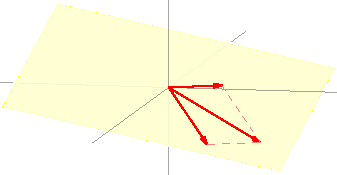
\includegraphics{asy/two_i_plane.pdf}    
\end{center}
\end{frame}\begin{frame}
For (1), take two members of the plane,
\begin{equation*}
  \vec{p}_1=\colvec{x_1 \\ y_1 \\ z_1}
  \quad
  \vec{p}_2=\colvec{x_2 \\ y_2 \\ z_2}
\end{equation*}
so that both $2x_1+y_1+3z_1=0$ and $2x_2+y_2+3z_2=0$.
The sum is 
\begin{equation*}
  \vec{p}_1+\vec{p}_2=\colvec{x_1+x_2 \\ y_1+y_2 \\ z_1+z_2}
\end{equation*}
and this sum is in the plane because it satisfies the
restriction.
\begin{equation*}
2(x_1+x_2)+(y_1+y_2)+3(z_1+z_2)=(2x_1+y_1+3z_1)+(2x_2+y_2+3z_2)=0
\end{equation*}
\end{frame}\begin{frame}
For condition~(6) take a member of the plane
\begin{equation*}
  \vec{p}=\colvec{x \\ y \\ z}
  \qquad 
  2x+y+3z=0
\end{equation*}
and multiply by a scalar $r\in\Re$. 
\begin{equation*}
  r\vec{p}=\colvec{rx \\ ry \\ rz}
\end{equation*}
Then $r\vec{p}$ is a member of the plane~$P$ because
$2(rx)+(ry)+3(rz)=r(2x+y+3z)=0$.
\end{frame}


\begin{frame}
\frametitle{$\Re^n$}
The set of $n$-tall vectors is a vector space under the 
natural operations.

All ten conditions are easy;  
we will just verify condition~(1).
Where
\begin{equation*}
  \vec{v}=\colvec{v_1 \\ \vdots \\ v_n}
  \qquad
  \vec{w}=\colvec{w_1 \\ \vdots \\ w_n}
\end{equation*}
then the sum
\begin{equation*}
  \vec{v}+\vec{w}
    =\colvec{v_1+w_1 \\ \vdots \\ v_n+w_n}
\end{equation*}
is also a member of $\Re^n$.
(There are no restrictions to check, since every $n$-tall vector is a 
member of $\Re^n$.)
\end{frame}

% ..........
\begin{frame}
\ex
Consider the set of quadratic polynomials.
\begin{equation*}
  \polyspace_2=\set{a_0+a_1x+a_2x^2 \suchthat a_0,a_1,a_2\in\Re}
\end{equation*}
Some members are $3+2x+1x^2$, $10+0x+5x^2$, and $0+0x+0x^2$.
\pause
This is a vector space under the usual operations of polynomial addition
\begin{equation*}
  (a_0+a_1x+a_2x^2)+(b_0+b_1x+b_2x^2)=(a_0+b_0)+(a_1+b_1)x+(a_2+b_2)x^2
\end{equation*}
and scalar multiplication.
\begin{equation*} 
r\cdot (a_0+a_1x+a_2x^2)=(ra_0)+(ra_1)x+(ra_2)x^2
\end{equation*}

Remember the intuition that a vector space is a place where linear
combinations can happen.
Here is a sample combination in $\polyspace_2$
\begin{equation*}
  4\cdot(1+2x+3x^2)-(1/5)\cdot (10+5x^2)
  =2+8x+11x^2
\end{equation*}
illustrating that 
a linear combination of quadratic polynomials is a quadratic polynomial.
\end{frame}\begin{frame}
We won't give a full verification but
we will check the closure conditions (1) and~(6).

For (1) note that if 
$\vec{v}=a_0+a_1x+a_2x^2$ and 
$\vec{w}=(b_0+b_1x+b_2x^2)$
then $\vec{v}+\vec{w}=(a_0+b_0)+(a_1+b_1)x+(a_2+b_2)x^2$ is also a quadratic
polynomial.

\pause
Similarly, for (6) note that
if $\vec{v}=a_0+a_1x+a_2x^2$ then
$r\cdot \vec{v}=(ra_0)+(ra_1)x+(ra_2)x^2$
is also a member of $\polyspace_2$.
\end{frame}



\begin{frame}
\ex
The set of $\nbyn{3}$ matrices
\begin{equation*}
  \matspace_{\nbyn{3}}=\set{\begin{mat}
                            a_{1,1}  &a_{1,2} &a_{1,3} \\
                            a_{2,1}  &a_{2,2} &a_{2,3} \\
                            a_{3,1}  &a_{3,2} &a_{3,3}
                          \end{mat} 
                         \suchthat a_{i,j}\in\Re}
\end{equation*}
is a vector space under the usual matrix addition and scalar multiplication.
The check of the ten conditions is straightforward.

Here is a sample linear combination.
\begin{equation*}
  \begin{mat}
    1 &0 &1 \\
    2 &0 &2 \\
   -1 &3 &1/2
  \end{mat}
  -3\begin{mat}
    0 &0 &2 \\
    1 &1 &1 \\
    0 &4 &3/2
  \end{mat}
  =
  \begin{mat}
    1 &0  &-5 \\
   -1 &-3 &1 \\
   -1 &-9 &-4
  \end{mat}
\end{equation*}
\end{frame}


\begin{frame}
The empty set cannot be made a vector space, regardless of which operations
we use, because the definition requires that the space contains 
an additive identity.

\pause
\ex
The set consisting only of the two-tall zero vector
\begin{equation*}
  V=\set{\colvec{0  \\  0}}
\end{equation*}
is a vector space (under the usual vector addition and scalar multiplication
operations).
\begin{equation*}
  \colvec{0 \\ 0}+\colvec{0 \\ 0}=\colvec{0 \\ 0}
  \qquad
  r\cdot\colvec{0 \\ 0}=\colvec{0 \\ 0}
\end{equation*}

\df[df:TrivialVectorSpace]
\ExecuteMetaData[\vsdir vs1.tex]{df:TrivialVectorSpace}
\end{frame}




% ..........
\begin{frame}
\lm[lm:ElementaryPropertiesOfVectorSpaces]
\ExecuteMetaData[\vsdir vs1.tex]{lm:ElementaryPropertiesOfVectorSpaces}

\pause
\pf
\ExecuteMetaData[\vsdir vs1.tex]{pf:ElementaryPropertiesOfVectorSpaces0}
\qed
\end{frame}







\section{Subspaces and spanning sets}

% ..........
\begin{frame}{Subspace}
\df[df:Subspace]
\ExecuteMetaData[\vsdir vs1.tex]{df:Subspace}

\pause\smallskip
\ExecuteMetaData[\vsdir vs1.tex]{ProperSubspace}

\pause
\ex
We have seen that in the vector space $\Re^2$, the line $y=2x$ 
\begin{equation*}
  S=\set{\colvec{a \\ 2a} \suchthat a\in\Re}
   =\set{\colvec{1 \\ 2}\cdot a \suchthat a\in\Re}
\end{equation*}
is a subspace.
The operations are the ones from $\Re^2$, as required by the definition above.
Earlier, to show it is a vector space we checked the ten conditions from the 
definition.
The result below says that to check if something is a subspace there
is an easier way.

\pause
\ex
This subset of $\matspace_{\nbyn{2}}$ is a subspace. 
\begin{equation*}
  S=\set{\begin{mat}
           a  &b  \\
           a  &b
         \end{mat} \suchthat a,b\in\Re}
   =\set{\begin{mat}
           1  &0  \\
           1  &0
         \end{mat}\cdot a
         +\begin{mat}
           0  &1  \\
           0  &1
          \end{mat}\cdot b
         \suchthat a,b\in\Re}
\end{equation*}
Addition and scalar multiplication are the same as in 
$\matspace_{\nbyn{2}}$.
\end{frame}




% ..........
\begin{frame}
\ex
This is not a subspace of $\Re^3$.
\begin{equation*}
  T=\set{\colvec{x  \\ y  \\ z}\suchthat x+y+z=1}
\end{equation*}
It is a subset of $\Re^3$ but it is not a vector space.
One condition that it violates is that it is not closed under vector addition:
here are two elements of $T$ that sum to a vector that is not an element of 
$T$. 
\begin{equation*}
  \colvec{1  \\ 0  \\ 0}
  +\colvec{0 \\ 1 \\ 0}
  =\colvec{1 \\ 1 \\ 0}
\end{equation*}
(Another reason that it is not a vector space is that it does not satisfy
condition~(6).
Still another is that it does not contain the zero vector.)
\end{frame}




% ..........
\begin{frame}
\lm[th:SubspIffClosed]
\ExecuteMetaData[\vsdir vs1.tex]{lm:SubspIffClosed}

\pause\medskip
\iftoggle{showallproofs}{
  \ExecuteMetaData[\vsdir vs1.tex]{pf:SubspIffClosed0}
}{
  The book has the full proof.
  For the idea, recall that in the first example of a vector space 
  we remarked that 
  some of the conditions do not depend on the restriction.
  For instance, there $\vec{v}_1+\vec{v}_2$ equals $\vec{v}_2+\vec{v}_1$ 
  \begin{equation*}
    \colvec{x_1 \\ y_1}+\colvec{x_2 \\ y_2}
    =\colvec{x_1+x_2 \\ y_1+y_2}
    =\colvec{x_2+x_1 \\ y_2+y_1}
    =\colvec{x_2 \\ y_2}+\colvec{x_1 \\ y_1}
  \end{equation*}
  because the vector components are real number sums.
  Only the closure conditions need verification.
  Statements~(2) and~(3) above combine the closure conditions
  into a single one, to make the verification faster.
}
\end{frame}
\iftoggle{showallproofs}{
  \begin{frame}
  \pf[th:SubspIffClosed]
  \ExecuteMetaData[\vsdir vs1.tex]{pf:SubspIffClosed1}

  \pause
  The conditions for scalar multiplication are similar.
  \qed
  \end{frame}
}{}




% ..........
\begin{frame}
\ex
The vector space of quadratic polynomials
$\polyspace_2=\set{a_0+a_1x+a_2x^2\suchthat a_0,a_1,a_2\in\Re}$ has a subspace
comprised of the linear polynomials
$L=\set{b_0+b_1x\suchthat b_0,b_1\in\Re}$.
By the prior result, to verify that we need only check 
closure under linear combinations of two members.
\begin{equation*}
  r\cdot(b_0+b_1x)+s\cdot(c_0+c_1x)=(rb_0+sc_0)+(rb_1+sc_1)x
\end{equation*}
The right side is a linear polynomial with real coefficients, and so is a 
member of $L$.
Thus $L$ is a subspace of $\polyspace_2$.

\pause
\ex
Another subspace of $\polyspace_2$ is the set of quadratic polynomials
having three equal coefficients.
\begin{equation*}
  M=\set{a+ax+ax^2\suchthat a\in\Re}
   =\set{(1+x+x^2)\cdot a\suchthat a\in\Re}
\end{equation*}
Verify that it is a subspace by
considering a linear combination of two of its members
(under the inherited operations).
\begin{equation*}
  r\cdot(a+ax+ax^2)+s\cdot(b+bx+bx^2)
  =(ra+sb)+(ra+sb)x+(ra+sb)x^2
\end{equation*}
The result is a quadratic polynomial with three equal coefficients  
and so $M$ is closed under linear combinations.
\end{frame}




% ..........
\begin{frame}
The prior subspace example 
parametrizes the description.
\begin{equation*}
  M=\set{a+ax+ax^2\suchthat a\in\Re}
  = \set{(1+x+x^2)\cdot a\suchthat a\in\Re}
\end{equation*}
That proves to be a great way to understand vector spaces.

\smallskip
\ex
This subset of $\Re^3$ is a plane.
\begin{equation*}
  P=\set{\colvec{x  \\ y  \\ z}\suchthat 2x-y+z=0}
\end{equation*}
We could
verify that it is a subspace by checking that it is closed under 
linear combination, as above.
However, that's easier if we first parametrize.
\pause
Solve the one-equation linear system
$2x-y+z=0$ to express the leading variable~$x$
in terms of the free variables $y$ and~$z$.
\begin{equation*}
  P=\set{\colvec{(1/2)y-(1/2)z  \\ y  \\ z}\suchthat y,z\in\Re}  
   =\set{\colvec{1/2 \\ 1 \\ 0}y+\colvec{-1/2 \\ 0 \\ 1 }z\suchthat y,z\in\Re}  
\end{equation*}
\end{frame}
\begin{frame}
\noindent With the parametrized description
\begin{equation*}
  P=\set{y\colvec{1/2 \\ 1 \\ 0}+z\colvec{-1/2 \\ 0 \\ 1 }\suchthat y,z\in\Re}  
  \tag{$*$}
\end{equation*}
showing the subspace is closed under linear combinations is straightforward
(here, $r_1,r_2\in\R$).
\begin{multline*}
  r_1\cdot\big(y_1\colvec{1/2 \\ 1 \\ 0}+z_1\colvec{-1/2 \\ 0 \\ 1 }\big)
  +r_2\cdot\big(y_2\colvec{1/2 \\ 1 \\ 0}+z_2\colvec{-1/2 \\ 0 \\ 1 }\big)
     \\
  =(r_1y_1+r_2y_2)\cdot\colvec{1/2 \\ 1 \\ 0}
     +(r_1z_1+r_2z_2)\cdot\colvec{-1/2 \\ 0 \\ 1 }
\end{multline*}
Line~($*$)
describes each member of $P$ as a linear combination of the two vectors.
Verifying that $P$ is closed then just involves taking a linear combination of 
linear combinations.
Of course, that gives a linear combination.
\end{frame}



\begin{frame}
\ex To show that this is a subspace of $\matspace_{\nbyn{2}}$
\begin{equation*}
  Q = 
  \set{
    \begin{mat}
      a &b \\
      c &d
    \end{mat}
    \suchthat 
      \text{$a-b=0$ and $b-c=0$}}
\end{equation*}
treat that as a two-equation linear system and parametrize.
The leading variables are $a$ and~$b$, with free variables $c$ and~$d$.
\begin{equation*}
  Q = 
  \set{
    \begin{mat}
      c &c \\
      c &d
    \end{mat}
    \suchthat 
      c,d\in\Re}
  = 
  \set{
    c
    \begin{mat}
      1 &1 \\
      1 &0
    \end{mat}
    +d
    \begin{mat}
      0 &0 \\
      0 &1
    \end{mat}
    \suchthat 
      c,d\in\Re}
\end{equation*}
\pause
To show $Q$ is a subspace, use the lemma's clause~(2) by finding that a
linear combination of such matrices is such a matrix.
\begin{multline*}
    r_1\cdot\big(c_1
    \begin{mat}
      1 &1 \\
      1 &0
    \end{mat}
    +d_1
    \begin{mat}
      0 &0 \\
      0 &1
    \end{mat}
    \big)
    +r_2\cdot\big(c_2
    \begin{mat}
      1 &1 \\
      1 &0
    \end{mat}
    +d_2
    \begin{mat}
      0 &0 \\
      0 &1
    \end{mat}
    \big)
                                       \\
    =(r_1c_1+r_2c_2)\cdot
    \begin{mat}
      1 &1 \\
      1 &0
    \end{mat}
    +(r_1d_1+r_2d_2))
    \begin{mat}
      0 &0 \\
      0 &1
    \end{mat}
\end{multline*}
\end{frame}


% ..........
\begin{frame}{Span}
\df[df:Span]
\ExecuteMetaData[\vsdir vs1.tex]{df:Span}

\medskip
\ExecuteMetaData[\vsdir vs1.tex]{NotationForSpan}

\pause
\ex
Inside the vector space of all two-wide row vectors, the span of this 
one-element set
\begin{equation*}
  S=\set{\rowvec{1  &2}}
\end{equation*}
is this.
\begin{equation*}
  \spanof{S}
  =\set{\rowvec{a &2a}\suchthat a\in\Re}
  =\set{\rowvec{1 &2}a\suchthat a\in\Re}
\end{equation*}
\end{frame}




% ..........
\begin{frame}
\ex
This is a subset of $\Re^3$.
\begin{equation*}
  \hat{S}=\set{\colvec{1 \\ -1 \\ 0},
         \colvec{1 \\ 1 \\ 0}}
\end{equation*}
Any vector in the $xy$-plane is a member of the span $\spanof{S}$ because 
any such vector is a combination of the two;
for instance, this system has a solution
\begin{equation*}
  \colvec{3 \\ 2 \\ 0}=\colvec{1 \\ -1 \\ 0}c_1
                       +\colvec{1 \\ 1 \\ 0}c_2
\end{equation*}
(the top two rows gives a linear system with a unique solution).
\pause
But vectors not in the $xy$-plane are not in the span. 
For instance,
this system does not have a solution.
\begin{equation*}
  \colvec{-1 \\ -2 \\ -3}=\colvec{1 \\ -1 \\ 0}c_1
                       +\colvec{1 \\ 1 \\ 0}c_2
\end{equation*}
\end{frame}



% ..........
\begin{frame}
\ex
Here is another subset of $\Re^3$.
\begin{equation*}
  P=\set{\colvec{1 \\ 0 \\ 2},
         \colvec{0 \\ 2 \\ 1}}
\end{equation*}
Vectors in the span $\spanof{P}$ are combinations of the two, shown in red.
The span is a plane through the origin.
\begin{center}
  $\spanof{P}=\set{\colvec{1 \\ 0 \\ 2}\cdot s+\colvec{0 \\ 2 \\ 1}\cdot t
                    \suchthat s,t\in\R}$
  \qquad
  \vcenteredhbox{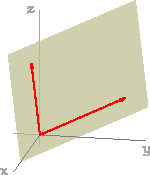
\includegraphics{asy/two_i_spanplane.pdf}}
\end{center}
\end{frame}




% ..........
\begin{frame}
\lm[le:SpanIsASubsp]
\ExecuteMetaData[\vsdir vs1.tex]{lm:SpanIsASubsp}

\pause
\pf
\ExecuteMetaData[\vsdir vs1.tex]{pf:SpanIsASubsp}
\qed
\end{frame}
\begin{frame}
\ex
This illustrates that a span is closed under linear combinations.
Where 
\begin{equation*}
  \hat{S}=\set{\colvec{1 \\ -1 \\ 0},
         \colvec{1 \\ 1 \\ 0}}\subset\Re^3
\end{equation*}
these are two elements of the span $\spanof{\hat{S}}$.
\begin{equation*}
  \vec{v}_1=5\cdot\colvec{1 \\ -1 \\ 0}
   +3\cdot\colvec{1 \\ 1 \\ 0}
  \qquad
  \vec{v}_2=-2\cdot\colvec{1 \\ -1 \\ 0}
    +10\cdot\colvec{1 \\ 1 \\ 0}
\end{equation*}
The linear combination of those two $-3\vec{v}_1+7\vec{v_2}$
makes another element of the span.
\begin{equation*}
  -3\cdot\big( 5\colvec{1 \\ -1 \\ 0}
   +3\colvec{1 \\ 1 \\ 0}\big)
  +7\cdot\big(-2\colvec{1 \\ -1 \\ 0}
    +10\colvec{1 \\ 1 \\ 0}\big)
  =
  -29\cdot\colvec{1 \\ -1 \\ 0}
    +61\colvec{1 \\ 1 \\ 0}
\end{equation*}
This is just an instance of
the Linear Combination Lemma: a linear combination of 
linear combinations is a linear combination. 
\end{frame}





% =============================================
\section{Spaces and their subspaces}
% ..... Two.I.2.19 .....
% \section{Real three-space}
\begin{frame}{Subspaces of $\Re^3$}
The next slide shows a sample of subspaces of the vector space~$\Re^3$:
the entire space, planes, lines, and the trivial subspace.
Subsets are drawn connected to supersets, on the levels 
directly above and below.

On the level one up from the bottom, the subspaces are lines 
(in the second and third case, because
the conjunction of the two conditions means that each is the 
intersection of two planes).
That is, they are one-dimensional.

On the next level up, the subspaces are planes, two-dimensional.
On the top level, the space is $3$-space.
\end{frame}

\begin{frame}
{\centering\includegraphics{asy/r3_subspaces.pdf}}  
\end{frame}


\begin{frame}{Express subspaces as spans}
\ex This is a subset of $\R^3$.
\begin{equation*}
  P=\set{\colvec{x \\ y \\ z}\suchthat x+y+z=0}
\end{equation*}
Here are three members of this set, and an equation showing that the third is a linear combination of the first two,
illustrating that it is a vector space.
\begin{equation*}
  \vec{v}_1=\colvec{1 \\ 2 \\ -3},
  \vec{v}_2=\colvec{-2 \\ -5 \\ 7},
  \vec{v}_3=\colvec{1 \\ 1 \\ -2},
  \qquad
  3\vec{v}_1+\vec{v}_2=\vec{v}_3
\end{equation*}

To get a more useful description, 
take the condition $x+y+z=0$ to be a one-equation linear system
and parametrize.
\begin{equation*}
  P=\set{\colvec{-y-z \\ y \\ z}\suchthat y,z\in\Re}
   =\set{\colvec{-1 \\ 1 \\ 0}y+\colvec{-1 \\ 0 \\ 1}z\suchthat y,z\in\Re}
\end{equation*}
Thus the plane is the span of those two vectors.
\end{frame}
\begin{frame}
The subspace~$P\subseteq\R^3$ is
a plane passing through the origin. 
\begin{center}
  $P=\spanof{\,\set{\colvec{-1 \\ 1 \\ 0}, 
            \colvec{-1 \\ 0 \\ 1}}\,}$
  \qquad
  \vcenteredhbox{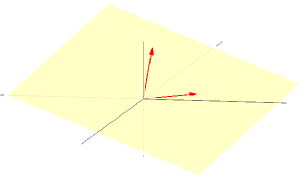
\includegraphics{asy/two_i_a_plane.pdf}}
\end{center}
The two vectors from the spanning set 
\begin{equation*}
  \colvec{-1 \\ 1 \\ 0} 
  \quad\text{and}\quad 
  \colvec{-1 \\ 0 \\ 1}
\end{equation*}
are in red.
For each, its entire body lies in the plane.
\end{frame}



\begin{frame}
\ex 
For the plane
\begin{equation*}
  \hat{P}=\set{\colvec{x \\ y \\ z}\suchthat x+2z=0}
\end{equation*}
repeat the process
\begin{equation*}
  \hat{P}=\set{\colvec{-2z \\ y \\ z}\suchthat y,z\in\Re}
         =\set{\colvec{0 \\ 1 \\ 0}y+\colvec{-2 \\ 0 \\ 1}z\suchthat y,z\in\Re}
\end{equation*}
to express it as a span.
\begin{equation*}
  \hat{P}=\spanof{\,\set{\colvec{0 \\ 1 \\ 0},
                         \colvec{-2 \\ 0 \\ 1}}\,}
\end{equation*}

\pause
\ex
The $xy$-plane is a span in a natural way.
\begin{equation*}
  \text{$xy$~plane}=\spanof{\,\set{\colvec{1 \\ 0 \\ 0},
                                   \colvec{0 \\ 1 \\ 0}}\,}
\end{equation*}
\end{frame}



\begin{frame}
\ex
Next we parametrize the lines.
The conditions in the set description
\begin{equation*}
  L=\set{\colvec{x \\ y \\ z}\suchthat \text{$x-y+z=0$ and $x+2z=0$}}
\end{equation*}
make a linear system.
\begin{equation*}
  \begin{linsys}{3}
    x &- &y &+ &z  &= &0 \\
    x &  &  &+ &2z &= &0
  \end{linsys}
  \grstep{-\rho_1+\rho_2}
  \begin{linsys}{3}
    x &- &y &+ &z  &= &0 \\
      &  &y &+ &z  &= &0
  \end{linsys}
\end{equation*}
Parametrizing
\begin{equation*}
  L=\set{\colvec{x \\ y \\ z}\suchthat \text{$y=-z$ and $x=-2z$}}
\end{equation*}
gives this.
\begin{equation*}
  L=\set{\colvec{-2 \\ -1 \\ 1}z\suchthat z\in\Re}
   =\spanof{\,\set{\colvec{-2 \\ -1 \\ 1}}\,}
\end{equation*}
\end{frame}
\begin{frame}
Here the line, the subspace, is  in yellow. 
\begin{center}
  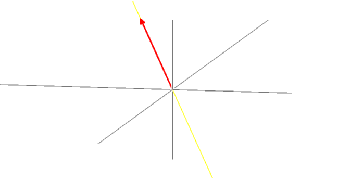
\includegraphics{asy/two_i_a_line.pdf}
\end{center}
In red is the vector used in the description.
\begin{equation*}
  \colvec{-2 \\ -1 \\ 1}
\end{equation*}
Its endpoint lies behind the plane of the screen, in the
octant where $x$ and~$y$
are negative and $z$ is positive.
\end{frame}


\begin{frame}
\ex
The line
\begin{equation*}
  \hat{L}=\set{\colvec{x \\ y \\ z}\suchthat \text{$y=2x$ and $z=0$}}
\end{equation*}
is easy to describe in a parametrized way.
\begin{align*}
  \hat{L} 
  &=\set{\colvec{1/2 \\ 1 \\ 0}y\suchthat y\in\Re}  \\
  &=\spanof{\,\set{\colvec{1/2 \\ 1 \\ 0}}\,}
\end{align*}

\pause
\ex
The $y$-axis is also easy to describe as a span.
\begin{equation*}
  \text{$y$-axis}
  =\spanof{\,\set{\colvec{0 \\ 1 \\ 0}}\,}
\end{equation*}
\end{frame}


\begin{frame}
\ex 
We can describe the entire space as a span.
\begin{equation*}
  \Re^3=\spanof{\,\set{\colvec{1 \\ 0 \\ 0},
                       \colvec{0 \\ 1 \\ 0},
                       \colvec{0 \\ 0 \\ 1}}\,}
\end{equation*}

\pause
\ex
We can do the same for the trivial subspace.
\begin{equation*}
  \set{\colvec{0 \\ 0 \\ 0}}
  =\spanof{\,\set{}\,}
\end{equation*}
(Remember that a sum of zero-many vectors 
is the zero vector.)
\end{frame}

\begin{frame}{$\Re^3$'s diagram reprised}
The following slide repeats the diagram of $\Re^3$'s subspaces, 
showing the same subspaces.
On this diagram the same subspaces they are described as spans, 
where the spanning set uses a minimal number of vectors.

By `minimal' we mean:~while 
we could describe the $xy$-plane in either of these ways,
\begin{equation*}
  \text{$xy$-plane}
  =\spanof{\,\set{\colvec{1 \\ 0 \\ 0},
                  \colvec{0 \\ 1 \\ 0}}\,}
  =\spanof{\,\set{\colvec{1 \\ 0 \\ 0},
                  \colvec{0 \\ 1 \\ 0},
                  \colvec{2 \\ -1 \\ 0}}\,}
\end{equation*}
the second has an extra vector, so the next slide doesn't use that description.
(We will soon make this precise.)

% \pause\medskip
% Note that 
% the subspaces fall naturally into levels, 
% depending on how many vectors are in a minimal spanning set.
\end{frame}
\begin{frame}
{\centering\includegraphics{asy/r3_subspaces_spans.pdf}}
\end{frame}




%...........................
% \section{The space of quadratic polynomials}
\begin{frame}{$\polyspace_2$'s subspaces}
The next slide has a picture of some of the subspaces of the
space of quadratic polynomials.
As with the $\Re^3$ diagram, 
subsets are shown connected to supersets on the adjacent level.

With $\Re^3$ the geometry gave us a good start for a natural classification
of subspaces into planes, lines, etc.
In this space there is less of that sense.
But there are a couple of natural subspaces.
\begin{align*}
  \text{linear polynomials}
    &=\set{0x^2+bx+c\suchthat b,c\in\Re}  \\
  \text{constant polynomials}
    &=\set{0x^2+0x+c\suchthat c\in\Re}  
\end{align*}
These are on the next slide, 
along with a couple of more-generic spaces.
\end{frame}
\begin{frame}
{\centering\includegraphics{asy/p2_subspaces.pdf}}  
\end{frame}


\begin{frame}{Parametrizing}
\ex
For the top level, this will do.
\begin{equation*}
  \polyspace_2
  =\spanof{\,\set{x^2,x,1}\,}
  =\spanof{\,\set{x^2+0x+0,
               0x^2+x+0,
               0x^2+0x+1}\,}       
\end{equation*}

\ex
On the bottom level, 
the trivial subspace is the span of the empty set.
\begin{equation*}
  \set{0}
  =\set{0x^2+0x+0}
  =\spanof{\,\set{}\,}
\end{equation*}

\pause
\ex
The set of linear polynomials has a natural expression as a span.
\begin{equation*}
 \set{bx+c\suchthat b,c\in\Re}
  =\spanof{\,\set{x,1}\,}
\end{equation*}

\ex
The set of constant polynomials is similar.
\begin{equation*}
  \set{0x^2+0x+c\suchthat c\in\Re}
  =\spanof{\,\set{1}\,}
\end{equation*}
\end{frame}


\begin{frame}
\ex
Parametrize $P=\set{ax^2+bx+c\suchthat a+b+c=0}$ 
in much the same way as for subspaces of real three-space:
treat the restriction as a one-equation linear system and parametrize.
\begin{align*}
  % \set{ax^2+bx+c\suchthat a+b+c=0}
  P
  &=\set{ax^2+bx+c\suchthat a=-b-c}     \\
  &=\set{(-b-c)\cdot x^2+bx+c\suchthat b,c\in\Re}  \\     
  &=\set{(-x^2+x)\cdot b+(-x^2+1)\cdot c\suchthat b,c\in\Re}       
\end{align*}
The spanning set is $\set{-x^2+x, -x^2+1}$.

\pause
\ex
Simliarly for 
$\hat{P}=\set{ax^2+bx+c\suchthat \text{$a-c=0$ and $b-c=0$}}$.
\begin{align*}
  \hat{P}
  &=\set{ax^2+bx+c\suchthat \text{$a=c$ and $b=c$}}     \\
  &=\set{cx^2+cx+c\suchthat c\in\Re}     \\
  &=\set{(x^2+x+1)\cdot c \suchthat c\in\Re}       
\end{align*}
The spanning set is $\set{x^2+x+1}$.

\pause\medskip
The next slide reprises $\polyspace_2$'s diagram,
with the subspaces described as spans.
\end{frame}
\begin{frame}
{\centering\includegraphics{asy/p2_subspaces_spans.pdf}}  
\end{frame}


% \section{Putting the examples together}
\begin{frame}
  \frametitle{Summary}

Subspaces are naturally described as spans.
In both examples these spans fall naturally into levels, 
according to the 
number of elements in a minimal spanning set. 

The book's next section gives a precise definition of 
when a spanning set is `minimal'.
The section after that shows that for any space, 
two minimal spanning sets have the same number of vectors.
\end{frame}



%...........................
% \begin{frame}
% \ExecuteMetaData[../gr3.tex]{GaussJordanReduction}
% \df[def:RedEchForm]
% 
% \end{frame}
\end{document}
